 \documentclass[11pt]{beamer}
\usepackage{amsfonts,amsmath,amsthm,amssymb}
\theoremstyle{plain}
\newtheorem{conjecture}{Conjecture}[section]
\usepackage{mathtools,mathptmx,listings,forest,enumitem}
\usepackage{graphicx}
\usepackage{pgfplots}
\pgfplotsset{compat=newest}
% plotting things
\usepackage{graphicx}
\graphicspath{{images/}}
\usepackage{tikz-cd}
\pgfplotsset{compat=1.15}
\usepackage[
	backend=biber,
	style=verbose,
	sorting=ynt
]{biblatex}
\addbibresource{references.bib}
\usetheme{Madrid}
\usepackage{float,mathtools,dirtytalk,ulem,csquotes,cancel,hyperref}
\usepackage{forest}
\usepackage{tikz-qtree}

\usepackage{tcolorbox}
\usepackage{subcaption}
\usepackage{quiver}

\author[] % (optional)
{Emon Hossain\inst{1}}

\institute[University of Dhaka] % (optional)
{
  \inst{1}%
  Lecturer\\MNS department\\Brac University
}

\date[] % (optional)
{\textsc{Lecture-01}}


\title[]{MAT215: Complex Variables And Laplace Transformations}

\setbeamertemplate{navigation symbols}{}


\AtBeginSection[]
{
  \begin{frame}
    \frametitle{Table of Contents}
    \tableofcontents[currentsection]
  \end{frame}
}

\usepackage{Kyushu}

% \usetheme{Frankfurt}

\begin{document}

\begin{frame}
\titlepage
\end{frame}

\begin{frame}{Motivation}
    You need motivation right? 
    \pause
    \begin{figure}
        \centering
        
\includegraphics[width=0.8\linewidth]{flop_motivation.png}
        \caption{\url{https://x.com/9gag/status/1051322203533430784}}
        % \label{fig:placeholder}
    \end{figure}
\end{frame}

\begin{frame}{Structures}

\begin{forest} for tree={
    edge path={\noexpand\path[\forestoption{edge}] (\forestOve{\forestove{@parent}}{name}.parent anchor) -- +(0,-12pt)-| (\forestove{name}.child anchor)\forestoption{edge label};}
}
[Structures
[Algebraic
[Field] [closed] [$\cdots$]
] 
[Geometric
[Metric] [$\cdots$]
]
[Topological]
 ] ]
\end{forest}
\end{frame}

\begin{frame}{Nothing to lose, only gain!}
    \begin{figure}
        \centering
        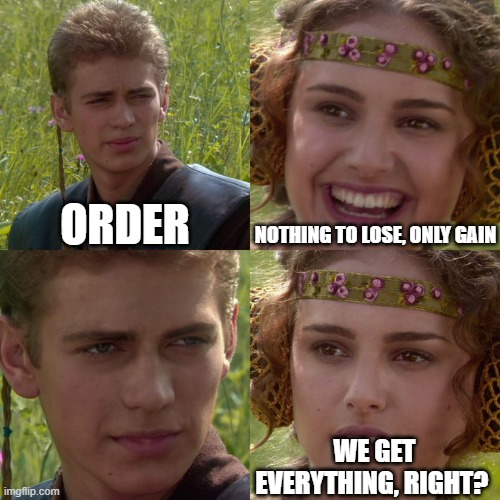
\includegraphics[width=0.6\linewidth]{only_gain.jpg}
    \end{figure}
    $$(i)+(-i)>0\qquad (i)+(-i)<0$$
\end{frame}

\begin{frame}{Imposter!}
        \begin{figure}[ht!]
    \centering
    
\includegraphics[width=0.6\linewidth]{com_me.jpg}
    \caption{Imposter}
    \label{fig:com_me}
\end{figure}
\end{frame}

\begin{frame}{Mate who cancel tours!}
    \begin{figure}[ht!]
    \centering
    
\includegraphics[width=0.7\linewidth]{i.jpg}
    \caption{$i$}
\end{figure}
\url{https://math.stackexchange.com/q/1760416/803654}
\end{frame}

\begin{frame}{Serious, study!}
    \begin{tcolorbox}
    Take $f:\mathbb R\rightarrow\mathbb R$, $$f(x)=\begin{cases}
        e^{-\frac{1}{x}},&x>0\\
        0, &x\leq 0
    \end{cases}$$  
    This function is smooth, but this is not analytic (Taylor expandable). Because $f^n=0$ for every $n$. So, the Taylor series about $0$ gives us $$f(0)+\sum_{n=1}^\infty\frac{f^n(0)}{n!}x^n=0\neq f(x)$$
    But this is not the case for functions with complex variables. Every smooth function on $\mathbb C$ is also analytic. 
    \end{tcolorbox}
\end{frame}

\begin{frame}{Continued...}
    \begin{tcolorbox}
        Consider the function, $$f(x)=\begin{cases}
            x^2\sin(1/x),&x\neq 0\\
            0, &x=0
        \end{cases}$$
        This function is once differentiable on $\mathbb R$, but the second derivative does not exist. However, for functions with complex variables, if a function is once differentiable, then it is infinitely differentiable.
    \end{tcolorbox}
\end{frame}

\begin{frame}{continued...}
The Analytic Miracle: Cauchy’s Integral Formula:
$$
f(z_0) = \frac{1}{2\pi i} \oint_{\gamma} \frac{f(z)}{z - z_0},dz
$$
\begin{quote}
    This means: to know a function inside a region, it is enough to know it only along the boundary. No other branch of analysis offers this generosity.    
\end{quote}
And:
\begin{quote}
   Differentiation and integration are no longer enemies — they become two faces of the same formula. 
\end{quote}
It’s almost as if the function remembers its boundary perfectly.
\begin{tcolorbox}
    Fundamental Theorem of Algebra: Every non-constant polynomial has a root in ($\mathbb{C}$).
\end{tcolorbox}
\end{frame}

\begin{frame}{Good-bye}
    \begin{figure}
        \centering
        
\includegraphics[width=0.5\linewidth]{qrcode.png}
    \end{figure}
\end{frame}
\end{document}